\chapter{Related Work}
There is a large body of active research on using the hand as an input modality
for human-computer interaction. To do this, the computer needs to be able to
interpret the dynamic and/or static configurations of the human hand, arm, and
even other parts of the human body. We break down the gestural input
system into several sequential modules shown in Figure \ref{fig:pipeline}.

\begin{figure}[h]
  \centering
  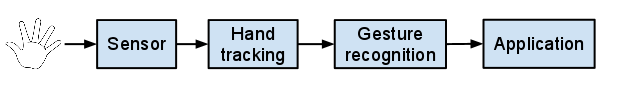
\includegraphics[width=0.7\textwidth]{figures/pipeline.png} 
  \caption{Gestural input pipeline.}
  \label{fig:pipeline}
\end{figure}

\section{Sensors}
The first step in the pipeline is having sensors that capture the hand movements
and configurations, converting analog signals to digital signals. First attempts
to solve this problem resulted in mechanical devices that directly measure hand
joint angles and spatial positions. This group is best represented by the
glove-based approaches using devices such us CyberGloves \cite{fels09} and
Powergloves \cite{kadous02}. However, wearing gloves makes gesturing more
cumbersome, and many efforts have been made to make the gloves more
light-weight, for example, by using Bluetooth wireless data transmission (e.g.,
CyberGove II). To further reduce the bulkiness of the gloves, people use colored
markers on the fingers \cite{mistry09} or colored gloves with no electronics \cite{Wang09}, and use RGB
cameras and computer vision techniques to interpret gestures. However, by
requiring the user to wear something extra still hinders the acceptance of
such devices as ``everyday'' natural interaction interfaces. 

The most non-obtrusive way to capture the hand is bare-hand tracking. Shin et
al. \cite{Shin04} use stereo RGB cameras to extract the hand from background based on the skin color. One
limitation of RGB cameras is that they are very sensitive to lighting
conditions. This prompted researchers to look into other types of cameras. Oka et al. 
\cite{Oka02} use thermal imaging for hand segmentation under complex
background and changing light, relying on the condition that a hand's
temperature is almost always distinct from the background. Their approach does
not detect finger contact with the surface. Larson et al. \cite{larson11}
improve on this method to detect the finger contact by using
the heat transferred from a user's hand to the surface for touch-based gestures.
However, in order to detect the heat trace, the user has to drag the fingers a
bit instead of just touching. This may be a small departure from what users
would expect as ``natural'' based on their experience in the physical world.

Thermal imaging measures radiation emitted by objects in the
\textit{far}-infrared (F-IR) spectrum. There are other well-known ``IR-imaging''
techniques used in the HCI community which use devices that operate in the \textit{near}-infrared (N-IR) spectrum.
N-IR is employed in some fairly recent interactive tabletop surfaces and depth
cameras. A number of projects in the HCI community have used IR for tabletop
interaction by detecting multi-touch gestures using an under mounted
camera and an illumination source. An example of this is Microsoft's 
Surface\textsuperscript{\textregistered}. Recently, portable multi-touch devices
such as phones and tablets have become more and more ubiquitous. These devices
are based on capacitive touch sensitive screens. Touch-based devices are
becoming more and more mature, however the kind of gestures one can use are still
limited. The gestures are usually limited in 2D space with one or multiple
fingers. 

Going beyond the limitation of touch-only gestures, researchers at Microsoft
augmented the Surface technology with a switchable diffuser, additional
strips of IR LEDS with a different wave length for diffuse illumination, and an
additional IR sensitive camera which images IR reflected from the diffuse
illumination of the environment \cite{hilliges09}. In this way, they can capture
the hand above the surface as well. The height of the hand is estimated based on
the pixel intensity.

Since the introduction of Kinect, a motion sensing input device by Microsoft for
the Xbox 360 video game console, researchers in the HCI community, as well as
many independent hackers, have been using Kinect's depth sensor for capturing
both body and hand gestures \cite{openni}. Since then, there are also many
similar devices coming into the market which have been used for capturing
gestures. For instance, Harrison et al. \cite{harrison11} use  a short-range
PrimeSense \cite{primesense} depth camera for their wearable multi-touch
interaction. In comparison to the aforementioned augmented Surface setup,
Kinect, and the likes, provide a cheap alternative for depth sensing. In this
thesis, we will explore the potential of using the Kinect sensor for detecting 
both the touch-based gesture and above-surface 3D gestures. Potentially, we can 
use the depth information for determining surface touch, and hence, eliminate
the need for the complicated electronics of a touch sensitive screen. This also 
enables the gestural interaction on a large tabletop display, much bigger than 
that of Microsoft's Surface.

\section{Hand Tracking}
After getting input from the sensor(s), the next step in the pipeline is
tracking the hand(s). This is essentially the frame-by-frame estimation of the
parameters of the hand model based on the sensor input. The complexity of the
hand model is application dependent. For a given application, a very coarse and
simple model may be sufficient. The simplest model is treating the hand as a
blob and only the 2D/3D location of the blob is tracked. For example, Sharma et
al. \cite{sharma00} use 2D positional and time differential parameters to track
the hands as blobs, which is sufficient for them to distinguish whether the
hands are doing a point, a contour, or a circle gesture. The PrimeSense NITE
middleware for OpenNI's natural interaction framework also tracks the hand as a
point. It requires the user to do a ``focus'' gesture (``click'' or ``wave'')
to gain control in order to start hand tracking \cite{primesense-manual}. The
gestures it supports are ``click'', ``wave'', ``swipe left'', ``swipe right'', 
``raise hand candidate'' and ``hand candidate moved''.

However, to make a more generalizable system for natural-like interaction, a
more sophisticated model is required. One step forward is adding fingertip
locations in the hand model as exemplified in \cite{Oka02} \cite{harrison11}
\cite{larson11}. Tracking fingertips is usually sufficient for manipulating
objects on the 2D surface. However, for a more rich set of gestures, the one
that also involves communicative gestures, we may need a more sophisticated
model. For instance, Wang et al. \cite{Wang09} uses a 26 DOF
3D skeletal model in their real-time hand-tracking system. 

Another approach is using an appearance-based model. This means that the model
parameters are not directly derived from the 3D spatial description of the hand.
The hand poses are modeled by relating the appearance of any pose to the 
appearance of the set of predefined, template poses \cite{Pavlovic97}. In
their markless hand-tracking system, Wang et al. \cite{wang11} use efficient
queries of a database of gestures and desktop-specific hand silhouette samples
for pinch/click gesture detection.

In our system, we propose a combination of both approaches. A simplified 3-D
skeletal hand model is useful for manipulative gestures because we want to know 
exactly where the fingertips are and the grabbing and releasing poses of the hand. For
communicative gestures, we just need to know the meaning of the gesture instead
of the exact spatial parameters. Hence example-based template models would be
more suitable which also require less computation.

\subsection{Gesture Spotting}
To distinguish unintentional movements from intentional
movements, a common approach is to use one or two nongesture HMMs to
provide likelihood thresholds for outlier rejection. For instance, in \cite{yang07}, a weak
universal movement model has been used for adaptive thresholding.
Peng et al. \cite{peng11} argue that using one or two HMMs cannot
effectively reject complex outliers, e.g., when they resemble portions of a
gesture. In addition to a general garbage gesture model, they train several
nongesture HMM models by automatically identifying and manually specifying nongesture models from the
training data. This approach is suitable when identifying dynamic communicative
gestures and when the set of the input data is limited. They only test on the
given dataset, but in real life the possible unintentional movements are
limitless and it is not clear how this approach will scale. In addition,
using nongesture HMMs only works for discrete communicative gestures, but not
for static or continuous manipulative gestures.

We will investigate the distinctions between unintentional and
intentional hand movements based on hand and arm poses and movements, and the
context of the interaction. The context of the interaction refers to the states
of the application, for examples, whether the user's hand is close to a movable
virtual object, or whether an object is selected and waits for further commands.

\section{Gesture Recognition}
Most gestural input applications have focused on tracking only
\cite{harrison11} \cite{larson11}. For hand gesture recognition, much of the
work is on synthetic gestures, most notably sign language recognition
\cite{Starner95} \cite{Bauer00} \cite{kadous02} \cite{Wang09}. For dynamic
gesture recognition, hidden Markov model (HMM) is a commonly used technique because it is suitable
for time series data \cite{sharma00}.

Elaborate more on \cite{Starner95}: embeded training: trains the models
\textit{in situ} and allows the boundaries to shift through a probabilistic
entry into the initial states of each model \cite{young1994}.

Wang et al. \cite{wang06} argue that a significant limitation of the
HMM is the requirement of conditional independence of observations. In
addition, HMM, as a generative model, optimizes the likelihood of
generating all the examples of a given gesture class, which is not
necessarily optimal for discriminating the gesture class against other
gestures. They introduced the use of hidden conditional random fields (HCRF),
an extension of conditional random fields (CRF), for gesture recognition, and
showed improved accuracy for the set of head and arm gestures they use in comparison to using HMMs. 
However, this approach does not handle continuous input. 

Morency et al. \cite{morency07} present a latent-dynamic conditional
random field (LDCRF) model that is able to perform sequence labeling and
segmentation simultaneously. However, their method only works for bounded
input sequences. Song et al. \cite{song12} extend LDCRF with multi-layered
filtering to make it work on unbounded input. However, their approach
still incurs some delay, e.g., one to four seconds in their experiments. For
real-time interaction, 0.1 second is about the limit for having the user feel
that the system is reacting instantaneously. We may relax this response time a
bit, but 1.0 second is about the limit for the user's flow of thought to stay
uninterrupted \cite{card91}.  Also they only focus on communicative
gestures and assume no unintentional gestures in the input data.

% Another limitation of CRF-based models is that training for these models is much
% more computationally expensive and converges much slower than those of HMMs 
% \cite{lafferty01}. To combine the benefits of both the HMM-based model and the 
% discriminative model, we propose to use discriminative training for the
% HMM-based model instead.

There is not much prior work that actually distinguishes manipulative gestures
and communicative gestures. Oka et al. \cite{Oka02} developed a system that
allows both direct manipulation and symbolic gestures. Based on the tracking result,
the system first differentiates the gesture as either manipulative or symbolic 
according to the extension of the thumb. They regard gestures with an extended 
thumb as direct manipulation and those with a bent thumb as symbolic gestures. 
For direct manipulation, the system selects operating modes such as rotate, 
move or re-size based on the fingertips configuration; for symbolic gestures, it 
uses HMM for classification. The way they distinguish manipulative and 
communicative gestures seems to be arbitrary and ``unnatural''. They did that 
probably for the ease of it because they are only tracking fingertips.
Instead, we propose an interface that can respond to manipulative and
communicative gestures seamlessly based on the inherent difference between the two.

Most prior works focus on recognizing one category of gestures: static hand
poses \cite{hu2013}, dynamic hand poses \cite{suryanarayan2010}, dynamic paths
\cite{song12}. Few work have looked into putting these together. People usually
use SVM for hand poses recognition. But SVM is useful when we have distinct hand
poses. This is not true for gestures with dynamic paths and poses.

We could conceivably just combine the two by first deciding what category the
gesture is and then apply different recognition methods. However making
decisions too early maybe not robust. Every stage there could be mistakes. So
making soft decisions rather than hard decisions and propagate the probabilities
until the very last stage when wen need to make the final decision. In this we
need to design the probabilistic inference system in a correct way, i.e. the
probabilities are comparable. If we use separate HMMs for gestures with dynamic
paths and SVM probability scores for gestures with static hand poses, it's not
clear how these probabilities can be compared with each other to allow us to
make the final decision. Hence we need to have a unified framework. 

\begin{lstlisting}
void LookForGesture() {
  // Swipe to right
  if (ScanPositions((p1, p2) => Math.Abs(p2.Y - p1.Y) < SwipeMaximalHeight, // Height
      (p1, p2) => p2.X - p1.X > -0.01f, // Progression to right
      (p1, p2) => Math.Abs(p2.X - p1.X) > SwipeMinimalLength, // Length
      SwipeMininalDuration, SwipeMaximalDuration)) // Duration {
    RaiseGestureDetected("SwipeToRight");
    return;
  }

  // Swipe to left
  if (ScanPositions((p1, p2) => Math.Abs(p2.Y - p1.Y) < SwipeMaximalHeight,  // Height
      (p1, p2) => p2.X - p1.X < 0.01f, // Progression to right
      (p1, p2) => Math.Abs(p2.X - p1.X) > SwipeMinimalLength, // Length
      SwipeMininalDuration, SwipeMaximalDuration))// Duration
        {
    RaiseGestureDetected("SwipeToLeft");
    return;
  }
}
\end{lstlisting}

\section{Kinect SDK}
The gesture interaction provided by the Kinect-based games and the Kinect SDK is
one of the popular ones. For Kinect games, a user starts by waving to the sensor
and then the sensor starts to track the user's hands, and at this point onwards,
the hand functions like a mouse. Then the sensor also looks for a specific
body pose (Figure. \ref{fig:kinect-pose}) to signal that the user wants to exit.
Notice that in this way, the system is only looking for one gesture or body pose at a time and the rest of
the time, it is just tracking the hand.

Kinect based controls are gestures that require continuous response.

\begin{figure}
\centering
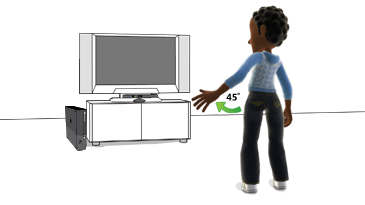
\includegraphics{figures/kinect_pose.png}
\caption{}
\label{fig:kinect-pose}
\end{figure}

\section{Leap Motion}
The gestures currently supported are:

1 to 2 fingers

Pointer � Point to anything on screen. Move your finger past the device to expand the pointer.

1 hand + 3 or more fingers (left/right/up/down)

Navigate through your slides. See config options to invert movements.

2 hands upwards

Toggle the overview mode. Do it a second time to exit the overview.

\begin{lstlisting}
// Gestures
    if( frame.gestures.length > 0 && (now - lastGesture) > config.gestureDelay ) {
      var gesture = frame.gestures[0];

      // One hand gestures
      if( frame.hands.length === 1 ) {
        // Swipe gestures. 3+ fingers.
        if( frame.fingers.length > 2 && gesture.type === 'swipe' ) {
          // Define here since some gestures will throw undefined for these.
          var x = gesture.direction[0],
              y = gesture.direction[1];

          // Left/right swipe gestures
          if( Math.abs( x ) > Math.abs( y )) {
            if( x > 0 ) {
              config.naturalSwipe ? Reveal.left() : Reveal.right();
            }
            else {
              config.naturalSwipe ? Reveal.right() : Reveal.left();
            }
          }
          // Up/down swipe gestures
          else {
            if( y > 0 ) {
              config.naturalSwipe ? Reveal.down() : Reveal.up();
            }
            else {
              config.naturalSwipe ? Reveal.up() : Reveal.down();
            }
          }

          lastGesture = now;
        }
      }
      // Two hand gestures
      else if( frame.hands.length === 2 ) {
        // Upward two hand swipe gesture
        if( gesture.direction[1] > 0 && gesture.type === 'swipe' ) {
          Reveal.toggleOverview();
        }

        lastGesture = now;
      }
    }
\end{lstlisting}

simple reflex agent based on if-then rules (condition-action rule) \cite{russell1996}
\section{Multi-modal Systems}
Bolt's pioneering work in the ``Put That There'' system \cite{Bolt80} 
demonstrated the potential for voice and gestural interaction.  In that system, 
the hand position and orientation were tracked by the Polhemus tracker, i.e.,
the hand was essentially transformed to a point on the screen. The actual hand 
posture did not matter, even if it was not in a pointing shape. The speech also 
followed a rigid and limited command-like grammar. Even though this is early 
work, it provides some insight about the advantages of multi-modal interaction. 
As Bolt summarized in the paper, using pointing gesture allows the use of 
pronouns in the speech, with the corresponding gain in naturalness and economy 
of expression \cite{Bolt80}.

Since then, several multi-modal interaction prototypes were 
developed that moved beyond Bolt's ``Put That There'' system. Cohen et al. 
\cite{Cohen97} developed the QuickSet prototype which is a collaborative, 
multi-modal system running on a hand-held PC using pen and voice as input. They 
used a novel multi-modal integration strategy that allows speech and pen gesture 
to compensate for each other, yielding a more robust system. Rauschert et al. 
\cite{Rauschert02} developed a system called Dialogue-Assisted Visual 
Environment for Geoinformation (DAVE\_G) that uses free hand gestures and speech
as input. They recognized that gestures are more useful for expressing spatial 
relations and locations. Gestures in DAVE\_G include pointing, indicating an 
area and outlining contours. Speech and gesture are fused for commands that need
spatial information provided by the gesture. 

In this thesis, we will also explore the fusion of speech and gestures. In
addition to using deictic gestures to provide spatial information as a
complement to speech as in \cite{Rauschert02}, we will explore the use of speech as a
complement to manipulative gestures based on the finding from the user study
done by Yin et al.\cite{yin10}. They observe that manipulative gestures are at times
accompanied by adjectives and adverbs that refine the actions.

control mouse

Data fusion
Result from ChaLearn \cite{escalera2013} shows that the top ranked three teams
all used late fusion of audio and skeleton data.
